\documentclass[12pt]{article}
\author{David Alves}

\usepackage{amsfonts}
\usepackage{amsmath}
\usepackage{amsthm}
\usepackage{dirtytalk}
\usepackage[a4paper, total={6.5in, 8.75in}]{geometry}
\usepackage{forest}
\usepackage{listings}
\usepackage{skak}
\usepackage{tikz}
\usepackage{titling}
\usepackage{wrapfig}
\usepackage{xcolor}

\usetikzlibrary{decorations.pathreplacing}
\usetikzlibrary{patterns}

\pgfdeclarepatternformonly{bigger north west lines}{\pgfqpoint{-2pt}{-2pt}}{\pgfqpoint{8pt}{8pt}}{\pgfqpoint{6pt}{6pt}}%
{
  \pgfsetlinewidth{1pt}
  \pgfpathmoveto{\pgfqpoint{0pt}{6pt}}
  \pgfpathlineto{\pgfqpoint{6.2pt}{-0.2pt}}
  \pgfusepath{stroke}
}

\def\multichoose#1#2{\ensuremath{\left(\kern-.3em\left(\genfrac{}{}{0pt}{}{#1}{#2}\right)\kern-.3em\right)}}

\newcommand{\ProblemStatement}[1]{
\subsection*{Problem Statement}
#1
\subsection*{Solution}
}

% If uncommented, next line hides problem statements 
%\renewcommand{\ProblemStatement}[1]{}


\title{Math 142 Problem Set 6}
\author{David Alves}
\date{2016-10-13}

\begin{document}
\pagenumbering{gobble}

\begin{center}
\large \thetitle \\
\theauthor \\
\thedate
\end{center}

\subsection*{Sources}

    \begin{itemize}
    \item http://tex.stackexchange.com and https://www.sharelatex.com for help with \LaTeX
    \item Wikipedia and math.stackexchange.com for a refresher on implication and logical equivalence.
    \end{itemize}

\section{Disjoint Tuples}
\ProblemStatement{
Fix positive integers $n$ and $k$, and let $S = [n]$. Find the number of $k$-tuples $(T_1, T_2, \ldots, T_k)$ of subsets $T_i$ such that $T_i$ are pairwise disjoint.
}

There are $(k+1)^{n}$ different $k$-tuples of pairwise-disjoint subsets of $S$.

\begin{proof}
An element $e \in S$ can be present in at most one of the sets $T_1, T_2, \ldots, T_k$ since if $e$ was present in two sets then those two sets would not be disjoint. It's also possible that $e$ is not present in any of the sets in the $k$-tuple. Therefore there is a bijection between $k$-tuples of pairwise-disjoint subsets of $S$ and placing $n$ distinguishable balls into $k+1$ distinguishable bins (one bin per element in the $k$-tuple and one for \say{not present in the tuple}). This gives $(k+1)^{n}$ different $k$-tuples of pairwise-disjoint subsets of $S$.
\end{proof}

\section{Bipartite Graphs}
\ProblemStatement{
Call a graph \textbf{bipartite} if its vertices can be written as a disjoint
union $A \cup B$ such that edges only go between $A$ and $B$, and never between
two vertices in $A$ or two vertices in $B$. Show that a graph $G$ is bipartite if and only if there is \textbf{not} an odd-length cycle, namely a sequence of vertices $v_1, v_2, \ldots, v_k$ where $(v_1, v_2), (v_2, v_3), \ldots, (v_{k-1}, v_k), (v_k, v_1)$ are all edges in $G$ and $k$ is odd.
}

Let B(G) denote the statement that G is a bipartite graph and O(G) denote the statement that there exists a subgraph of G which is an odd-length cycle. In order to show that for all $G$,$B(G) \iff \neg O(G)$, we must show that for all $G$, $B(G) \implies \neg O(G)$ and for all $G$, $\neg O(G) \implies B(G)$.

\subsubsection*{Proof that for all G, $B(G) \implies \neg O(G)$}

\begin{proof}
We prove this by contradiction. Assume that (for all $G$, $B(G) \implies \neg O(G)$) is false. We can rewrite $\neg(B(G)\implies \neg O(G))$ as $\neg(\neg B(G)\vee \neg O(G))$  which simplifies to $B(G) \wedge O(G)$. Therefore to prove our assumption, we must show that there exists a graph $G$ such that $B(G)$ and $O(G)$ are true.

Let $G$ be a graph such that $B(G)$ and $O(G)$ are both true. Then there exists a vertex sequence $v_1, v_2, \ldots, v_k$ such that $k$ is odd and $(v_1, v_2), (v_2, v_3), \ldots, (v_{k-1}, v_k), (v_k, v_1)$ are edges in $G$, and disjoint vertex sets $A$ and $B$ exist such that all vertices are in $A$ or $B$. Without loss of generality, let $v_1 \in A$. Then $v_2 \in B$ since we know that edge $(v_1, v_2)$ exists and $v1 \in A$. Similarly $v_3$ must be in $A$ because $v_2 \in B$ and edge $(v_2, v_3)$ exists. This gives an alternating sequence of $A$ and $B$ memberships $v_1 \in A, v_2 \in B, v_3 \in A, v_4 \in B, \ldots$ such that $v_i \in A$ if and only if $i$ is odd. This means that $v_k \in A$ since $k$ is odd, which means that $(v_k, v_1)$ does not exist since $v_1$ and $v_k$ are both in $A$, but $O(G)$ states that $(v_k, v_1)$ exists. Thus no graph $G$ exists such that $B(G) \wedge O(G)$ , so our assumption must be false and  $B(G) \implies \neg O(G)$ for all $G$.
\end{proof}

\subsubsection*{Proof that for all G, $\neg O(G) \implies B(G)$}
\begin{proof}
We prove this by contradiction. Assume that (for all G, $\neg O(G) \implies B(G)$) is false. We can rewrite $\neg(\neg O(G)\implies B(G))$ as $\neg(O(G) \vee B(G))$  which simplifies to $\neg B(G) \wedge \neg O(G)$. Therefore to prove our assumption, we must show that there exists a $G$ such that $B(G)$ and $O(G)$ are false.

Arbitrarily number the vertices in $G$ as $v_1, v_2, \ldots, v_n$. Divide all vertices into disjoint sets $A$ and $B$ as follows:
    
    \[
    v_k \in 
    \begin{cases} 
      A:& d(v_1, v_k) \text{ even (including when } k = 1 \text{ since }d(v_1, v_1) = 0)\\
      B:& d(v_1, v_k) \text{ odd}\\
    \end{cases}
    \]    
    where $d(v_i, v_j)$ is defined as the shortest-path distance from $v_i$ to $v_j$. We know that after doing this there must be some $v_i, v_j \in G$ such that $(v_i, v_j) \in G$ and $v_i, v_j$ are both in the same set because otherwise we have shown that $G$ is bipartite. But if $v_i$ and $v_j$ are in the same set then $d(v_1, v_i)$ and $d(v_1, v_j)$ are either both even or both odd, so their sum is even. Since $(v_i, v_j)$ exists in the graph, there is an odd-length cycle: 
    \[
%        (v_i, v_j) + \text{ path from } v_j \text{ to } v_1 + \text{ path from v_1 to v_i }) 
        (v_i, v_j) + \text{ (path from } v_j \text{ to } v_1) + \text{ (path from } v_1 \text{ to } v_i)
    \]
    This contradicts our assumption that there are no odd-length cycles in $G$, so there is no graph $G$ such that $\neg B(G) \wedge \neg O(G)$, so our assumption must be false and therefore $\neg O(G) \implies B(G)$ for all $G$.
\end{proof}


\section{Fibonacci Squares}
\ProblemStatement{
Prove the identity that $\sum_{i=0}^{n} (a_i)^2 = a_na_{n+1}$ where $a_n$ is the $n$-th Fibonacci number. For example, \[
    1^2 + 1^2 + 2^2 + 3^2 + 5^2 = 40 = 5 * 8
\]
}

\begin{proof}
We prove this by induction. Let $p(n)$ be the statement $\sum_{i=0}^{n}
(a_i)^2 = a_na_{n+1}$. For $n = 0$, we have $(a_0)^2 = a_0a_1$ or $1^2 = 1 \times 1$, so $p(0)$ is true. Next we show that for $n \geq 0$ if $p(n)$ is true, then $p(n+1)$ is true. $p(n)$ is

\begin{equation}
    a_0^2 + a_1^2 + \ldots + a_{n-1}^2 + a_n^2 = a_na_{n+1}
\end{equation}
while $p(n+1)$ is 
\begin{equation}
    a_0^2 + a_1^2 + \ldots + a_n^2 + a_{n+1}^2 = a_{n+1}a_{n+2}
\end{equation}
We can then substitute equation 1 into equation 2, giving
\[
     a_na_{n+1} + a_{n+1}^2 = a_{n+1}a_{n+2}
\]
dividing by $a_{n+1}$ gives 
\[
     a_n + a_{n+1} = a_{n+2}
\]
which is true because it is the definition of the Fibonacci series. Therefore if $p(n)$ is true then $p(n+1)$ is true, which completes the proof.

\end{proof}

\begin{center}
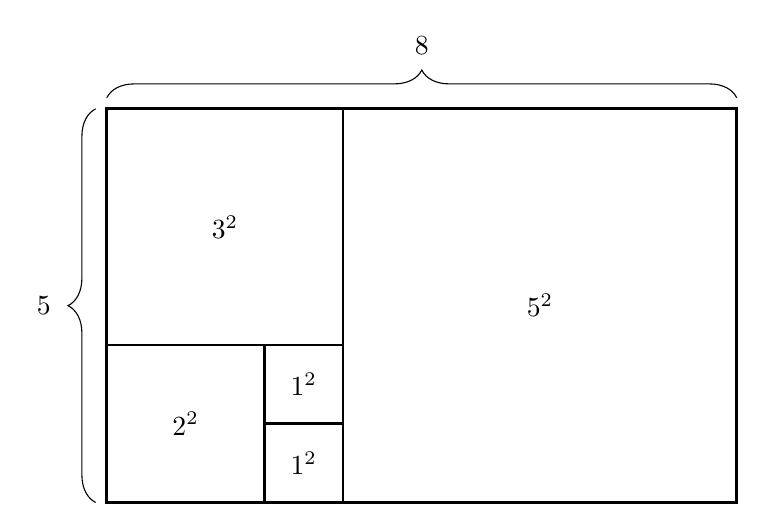
\begin{tikzpicture}

\draw[line width=1pt] (0,0) rectangle (-1,1);
\draw[line width=1pt] (0,1) rectangle (-1,2);
\draw[line width=1pt] (-1,0) rectangle (-3,2);
\draw[line width=1pt] (0,2) rectangle (-3,5);
\draw[line width=1pt] (0,0) rectangle (5,5);

\node at (-.5,.5) {$1^2$};
\node at (-.5,1.5) {$1^2$};
\node at (-2,1) {$2^2$};
\node at (-1.5,3.5) {$3^2$};
\node at (2.5,2.5) {$5^2$};
\draw [decorate,decoration={brace,amplitude=10pt,raise=4pt},yshift=0pt]
(-3,0) -- (-3,5) node [black,midway,xshift=-0.8cm] {5};
\draw [decorate,decoration={brace,amplitude=10pt,raise=4pt},yshift=0pt]
(-3,5) -- (5,5) node [black,midway,yshift=0.8cm] {8};

\end{tikzpicture}
\end{center}

\section{Trillary vs. Hump}
\ProblemStatement{
Suppose there are $2n$ anonymous votes to be tallied for Trillary vs. Hump in an important election, and you're looking at the votes one by one. Call a \emph{voting sequence} the sequence of votes you are seeing. (For example, there are four voting sequences for $n=1: TH, TT, HT, HH$, using abbreviations for candidate names). For each $n$, count the number of voting sequences there are such that both
\begin{itemize}
\item The votes are tied at the end with $n$ votes each.
\item At no point during your one-by-one examination of the votes is Hump ever ahead.
\end{itemize}
}

The number of voting sequences is the $n$\textsuperscript{th} Catalan number, $C_n$.
\begin{proof}
As you examine the votes, plot the partial results as follows:
\begin{itemize}
\item Start at (0,0)
\item As you examine each vote, increase the $x$ value by 1. If it is a vote for Trillary, increase the $y$ value by one, otherwise decrease the $y$ value by one. 
\item Connect the position before the current vote with the position after the current vote by a straight line.
\end{itemize}
The $y$ value for any $x$ is the number of votes that Trillary is leading by after the first $x$ votes have been counted. Since we are given that Hump is never ahead, the plot will never go below the $x$-axis. Since we are given that the votes are tied at the end, the final position will be $(2n,0)$. Thus there is a bijection between sequences of votes in this problem and the number of paths from $(0,0)$ to $(2n,0)$ such that each step of the path moves by $(+1, +1)$ or $(+1, -1)$ and the path never goes below $x=0$. Therefore the number of voting sequences is the $n$\textsuperscript{th} Catalan number, $C_n$.
\end{proof}
\begin{center}
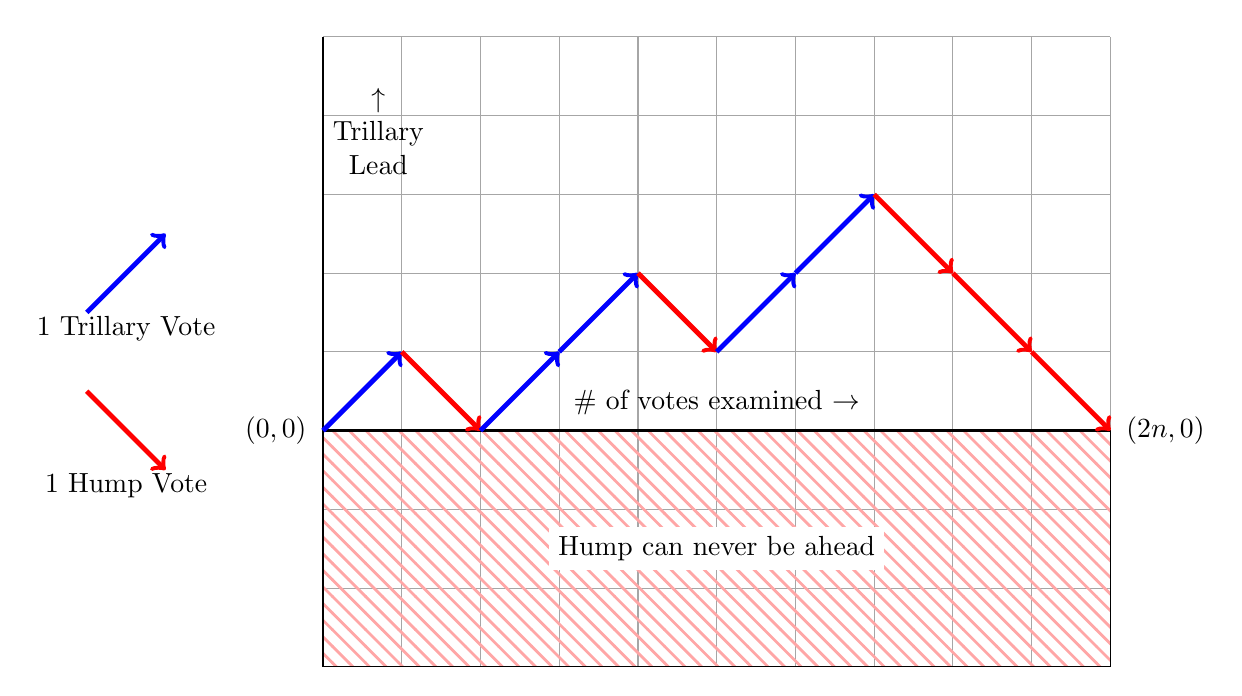
\begin{tikzpicture}
%\shade[bottom color=white, top color=blue,opacity=.2](-5,0) rectangle (5,5);
%\shade[top color=white, bottom color=red,opacity=.2](-5,0) rectangle (5,-5);
\draw[step=1.0,black,thin,color=black,opacity=.35] (-5,-3) grid (5,5);
\node (S) at (-5, 0) {};
\node (E) at (5, 0) {};
\node (T) at (-5, 5) {};

\draw[pattern=bigger north west lines, pattern color=red!35] (-5,0) rectangle (5,-3) node [midway,fill=white] {Hump can never be ahead};

\draw [-,line width=.9] (-5,-3) -- (-5,5) node [pos=.85,align=center,xshift=2em] {$\uparrow$\\Trillary\\Lead};
\draw [-,line width=.9] (-5,0) -- (5,0) node [midway,yshift=1em] {\# of votes examined $\rightarrow$};

\draw [->,line width=1.75,blue] (-8,1.5) -- (-7,2.5) node[midway, black, yshift=-2em] {1 Trillary Vote};
\draw [->,line width=1.75,red]  (-8,0.5) -- (-7,-.5) node[midway, black, yshift=-2em] {1 Hump Vote};

\draw [->,line width=1.75,blue] (-5,0) -- (-4,1);
\draw [->,line width=1.75,red] (-4,1) -- (-3,0);
\draw [->,line width=1.75,blue] (-3,0) -- (-2,1);
\draw [->,line width=1.75,blue] (-2,1) -- (-1,2);
\draw [->,line width=1.75,red] (-1,2) -- (0,1);
\draw [->,line width=1.75,blue] (0,1) -- (1,2);
\draw [->,line width=1.75,blue] (1,2) -- (2,3);
\draw [->,line width=1.75,red] (2,3) -- (3,2);
\draw [->,line width=1.75,red] (3,2) -- (4,1);
\draw [->,line width=1.75,red] (4,1) -- (5,0);
\node [black] at (-5.6,0) {$(0,0)$};
\node [black] at (5.7,0) {$(2n,0)$};

\end{tikzpicture}
\end{center}


\section{Computers \& Printers}
\ProblemStatement{
We have 10 distinguishable computers and 3 distinguishable printers. Each computer must be linked to exactly one printer. But if a printer has 8 or more computers linked to it, it will overheat. How many assignments of computers to printers are there such that we have no overheating?
}
 
There are 58446 ways to connect 10 printers to 3 printers without overheating.

\begin{proof}
There are three choices of printer for each computer, giving $3^{10}=59049$ possible assignments by the product principle. The total number of assignments is equal to the number of non-overheating assignments plus the number of assignments where a single printer has 8, 9, or 10 computers attached to it by the sum principle. Therefore we can subtract the overheating assignments from the total number of assignments to get the non-overheating assignments.

Three assignments cause overheating by connecting all 10 computers to the same printer. For connecting nine computers to a single printer, there are $\binom{10}{9} = 10$ ways to choose the 9 computers multiplied by 3 choices for the printer. For each of these there are two printer choices for the remaining computer, resulting in a total of $10 \times 3 \times 2 = 60$ assignments which overheat due to 9 computers on a single printer. Lastly, for 8 computers connected to a single printer there are $\binom{10}{8}=45$ ways to choose the 8 computers, 3 ways to choose the printer, and $2^2=4$ choices for the other two computers. 

Therefore we have a total of 
\[
    3^{10} - 3 - \binom{10}{9}\times3\times2 - \binom{10}{8}\times3\times2^2 = 58446
\]
ways to connect 10 computers to 3 printers without overheating.


\end{proof}


\section{Time Spent \& Thoughts}

How about some harder bijections / proofs that are related to the stuff we've been doing in class? This problem set seemed like four easy problems from class and one very hard problem unrelated to what we've done (the bipartite graphs / odd cycles proof). They all took about 15-30 minutes except that one, which took about 3-4 hours.

\end{document}
